% DriveAlert AI - Review 2
% Compile from the project root: tectonic -X compile main.tex
% Keep presentation_assets/ beside this file (screenshots, plots, measured data).
% The supplied 15-paper case study is summarized in one literature frame.
\PassOptionsToPackage{table}{xcolor}
\documentclass[aspectratio=169,10pt]{beamer}
\usetheme{Madrid}
% Larger 16:9 canvas accommodates the complete review in exactly 20 slides.
\geometry{paperwidth=224mm,paperheight=126mm}
\setbeamerfont{normal text}{size=\normalsize}
\definecolor{AmritaRed}{RGB}{169,29,58}
\definecolor{DarkSlate}{RGB}{30,41,59}
\definecolor{CardBg}{RGB}{241,245,249}
\definecolor{HighlightRed}{RGB}{254,242,242}
\setbeamercolor{palette primary}{bg=AmritaRed,fg=white}
\setbeamercolor{palette secondary}{bg=DarkSlate,fg=white}
\setbeamercolor{palette tertiary}{bg=AmritaRed,fg=white}
\setbeamercolor{frametitle}{bg=AmritaRed,fg=white}
\setbeamercolor{structure}{fg=AmritaRed}
\setbeamercolor{block title}{bg=AmritaRed,fg=white}
\setbeamercolor{block body}{bg=CardBg,fg=black}
\setbeamercolor{block title example}{bg=DarkSlate,fg=white}
\setbeamercolor{block body example}{bg=CardBg,fg=black}
\setbeamertemplate{blocks}[rounded][shadow=false]
\setbeamertemplate{navigation symbols}{}
\setbeamertemplate{headline}{}
\setbeamertemplate{itemize items}[circle]
\setbeamertemplate{enumerate items}[default]
\setbeamersize{text margin left=0.55cm,text margin right=0.55cm}
\usepackage{booktabs,tabularx,array,graphicx,amsmath,amssymb,tikz,pgfplots}
\usetikzlibrary{arrows.meta,positioning,calc}
\pgfplotsset{compat=1.18}
\hypersetup{colorlinks=true,urlcolor=AmritaRed,linkcolor=AmritaRed,pdftitle={DriveAlert AI - Review 2},pdfauthor={DriveAlert Team}}
\graphicspath{{presentation_assets/}}
\newcolumntype{Y}{>{\raggedright\arraybackslash}X}
\newcolumntype{L}[1]{>{\raggedright\arraybackslash}p{#1}}
\renewcommand{\arraystretch}{1.22}
\setlength{\tabcolsep}{5pt}
\newcommand{\src}[1]{\par\vfill\vspace{1mm}{\fontsize{6.5}{7.3}\selectfont\color{DarkSlate}#1\par}}
\newcommand{\smallnote}[1]{{\footnotesize\color{DarkSlate}#1\par}}
\newcommand{\headrow}{\rowcolor{CardBg}\bfseries}
\tikzset{flow/.style={execute at begin node={\hyphenpenalty=10000\exhyphenpenalty=10000},draw=DarkSlate,fill=CardBg,rounded corners=2pt,align=center,font=\footnotesize,minimum height=0.66cm,text width=2.55cm},arr/.style={-{Stealth[length=2mm]},thick,AmritaRed}}
\setbeamertemplate{footline}{%
 \hbox{%
 \begin{beamercolorbox}[wd=.65\paperwidth,ht=2.7ex,dp=1.2ex,leftskip=0.5cm]{palette primary}\scriptsize Amrita Vishwa Vidyapeetham\enspace /\enspace CSE Department\end{beamercolorbox}%
 \begin{beamercolorbox}[wd=.35\paperwidth,ht=2.7ex,dp=1.2ex,rightskip=0.5cm plus 1fil]{palette secondary}\hfill\scriptsize Review 2\enspace\insertframenumber/\inserttotalframenumber\end{beamercolorbox}}
}
\newcommand{\MedianLatency}{94.31}
\newcommand{\PninetyfiveLatency}{99.66}

\title{DriveAlert AI}
\subtitle{Real-Time Driver Fatigue and Microsleep Detection for Commercial Transport Safety}
\author{Group 13}
\institute{Amrita Vishwa Vidyapeetham}
\date{Review 2}
\hypersetup{pdftitle={DriveAlert AI: Real-Time Driver Fatigue and Microsleep Detection for Commercial Transport Safety},pdfauthor={Group 13}}
\begin{document}

% 1 - Cover; counted within the 20-slide total.
\begin{frame}[plain,t]
\centering
\vspace{5mm}
{\fontsize{11}{13}\selectfont\color{DarkSlate}Amrita Vishwa Vidyapeetham\par CSE Department\par}
\vspace{4mm}
{\bfseries\fontsize{30}{34}\selectfont\color{AmritaRed}DriveAlert AI\par}
\vspace{2mm}
{\bfseries\fontsize{19}{23}\selectfont\color{DarkSlate}Real-Time Driver Fatigue and Microsleep Detection\par for Commercial Transport Safety\par}
\vspace{4mm}
{\fontsize{11}{14}\selectfont\color{AmritaRed}AI-powered vigilance for every mile:\par preventing fatigue, protecting lives\par}
\vspace{5mm}
{\fontsize{13}{16}\selectfont\bfseries Review 2\enspace /\enspace Group 13\par}
\vspace{5mm}
\begin{columns}[T,onlytextwidth]
\column{.32\textwidth}\centering
\textbf{Krishnan S}\par
CB.SC.U4CSE23628\par\vspace{2pt}
{\footnotesize MobileNetV3-Small: deployment model\par}
\column{.32\textwidth}\centering
\textbf{Adwaith Raveendran}\par
CB.SC.U4CSE23603\par\vspace{2pt}
{\footnotesize EfficientNet-B0: efficiency comparison\par}
\column{.32\textwidth}\centering
\textbf{Eric Febin}\par
CB.SC.U4CSE23717\par\vspace{2pt}
{\footnotesize ResNet-18: accuracy benchmark\par}
\end{columns}
\vspace{5mm}
{\fontsize{10}{12}\selectfont\textbf{21CSC302 Deep Learning / Capstone Project}\par
\textbf{Faculty guide:} Dr. Bagyammal T, Professor, CSE Department\par}
\vspace{4mm}
{\fontsize{9}{11}\selectfont A webcam-based prototype combining eye and mouth classification with context-aware temporal alerts.\par}
\vfill
{\fontsize{8}{10}\selectfont\href{https://github.com/krishnans4132/DriveAI}{github.com/krishnans4132/DriveAI}\par}
\vspace{2mm}
{\fontsize{7}{9}\selectfont\color{DarkSlate}Project scope: local webcam inference, simulated vehicle telemetry and a demonstration rest route.\par}
\vspace{3mm}
\note{Title and tagline follow the supplied Group-13(PPT), Review 1, cover. Explain that two separate MobileNet models run in the live application. The three architectures are evaluated as alternatives, not as an ensemble.}
\end{frame}

\begin{frame}[t]{Problem, Motivation and Objectives}
\fontsize{10}{11.5}\selectfont
\renewcommand{\arraystretch}{1.06}
\setlength{\tabcolsep}{4pt}
\setlength{\abovedisplayskip}{4pt}
\setlength{\belowdisplayskip}{4pt}
\fontsize{10}{11.5}\selectfont
\renewcommand{\arraystretch}{1.06}
\setlength{\tabcolsep}{3pt}
\setlength{\abovedisplayskip}{3pt}
\setlength{\belowdisplayskip}{3pt}
\begin{columns}[T,onlytextwidth]
\column{.49\textwidth}
\textbf{Problem statement}\par\vspace{1pt}
Commercial drivers face fatigue and microsleep risks during long driving hours and irregular work schedules. Costly sensors, infrared cameras and specialised hardware can limit access to driver monitoring. Changes in lighting, head pose and eyewear also challenge detection reliability.
\par\smallskip
DriveAlert aims to provide an affordable AI-based system that detects fatigue and microsleep in real time using a standard RGB camera, operates efficiently in driving conditions and gives timely warnings to help prevent accidents.
\par\medskip
\textbf{Motivation}\par\vspace{1pt}
\begin{itemize}\setlength\itemsep{2pt}
\item Reduce fatigue-related accident risk and protect commercial drivers, passengers and other road users.
\item Make driver monitoring affordable through a standard RGB camera and accessible hardware.
\item Use deep learning and computer vision to pursue accurate, real-time fatigue detection.
\item Provide immediate alerts that support early driver action and safer, smarter transportation.
\end{itemize}
\column{.49\textwidth}
\textbf{Objectives and application scope}\par\vspace{1pt}
\begin{enumerate}\setlength\itemsep{0pt}
\item Compare MobileNetV3-Small, EfficientNet-B0 and ResNet-18 on shared eye/mouth splits.
\item Extract consistent facial crops using MediaPipe, with an OpenCV fallback.
\item Combine eye-closure duration, a PERCLOS proxy and yawn-event frequency.
\item Adjust temporal alert thresholds using simulated speed and driving duration.
\item Display evidence, offer spoken warnings and show a simulated rest route.
\end{enumerate}
\par\vspace{1pt}
\textbf{Scope boundary}\par\vspace{1pt}
The classifier outputs facial states. The separate decision engine interprets those states over time. Speed and duration do not retrain the network or change its locked probability cutoffs.
\par
\end{columns}


\src{Problem and motivation adapted from Group-13(PPT), Review 1, slides 3--4. Safety, accuracy and real-world robustness are project aims, not demonstrated outcomes. Implemented scope: README.md; backend/app.py, model\_runtime.py and fatigue\_engine.py; src/components/SimulatorDashboard.jsx.}
\end{frame}

\begin{frame}[t]{15-Paper Literature Review (2025--2026) and Contribution}
\fontsize{10}{11.5}\selectfont
\renewcommand{\arraystretch}{1.06}
\setlength{\tabcolsep}{4pt}
\setlength{\abovedisplayskip}{4pt}
\setlength{\belowdisplayskip}{4pt}
\small
\begin{tabularx}{\textwidth}{L{3cm} L{2.2cm} Y}
\toprule
\textbf{Member} & \textbf{Five papers} & \textbf{Main finding and remaining gap}\\\midrule
Krishnan S & [1, 2, 3, 10, 11] & Compact models support deployment; adaptive windows already exist. Lighting and device costs still matter.\\
Adwaith Raveendran & [4, 5, 6, 12, 13] & Temporal/multi-region methods enrich features; unseen-driver testing and matched runtime comparisons are needed.\\
Eric Febin & [7, 8, 9, 14, 15] & Fusion and explainability support monitoring; on-road validity and driver response remain insufficiently tested.\\\bottomrule
\end{tabularx}
\par\vspace{1pt}
\textbf{Selected standard paper [1]:} Vimala et al., \textit{Implementation of a lightweight deep learning model for detecting driver fatigue}, Franklin Open (2026).\par
\textbf{Why selected:} compares MobileNetV3-Small and EfficientNet variants for the same accuracy--resource tradeoff as DriveAlert. \href{https://doi.org/10.1016/j.fraope.2026.100547}{DOI: 10.1016/j.fraope.2026.100547}
\par\vspace{1pt}
\textbf{Project research question:} do speed and drive-duration rules improve alert delay and false alerts beyond fixed and confidence-adaptive baselines? This benefit remains to be tested.
\par\medskip
\textbf{Implemented contribution}\par\vspace{1pt}
A modular combination of compact eye/mouth CNNs, temporal evidence and speed/drive-duration-dependent decision thresholds, with visible alert reasons and local inference.
\par
\par\vspace{1pt}
\begin{itemize}\setlength\itemsep{0pt}
\item Two task-specific networks replace the standard classification outputs with 1 and 3 logits.
\item Context adapts the downstream policy while retaining validation-locked model thresholds.
\item Participant-separated comparison and transparent error reporting support reproducibility.
\end{itemize}
\par\vspace{1pt}
\textbf{Novelty boundary:} these are existing neural backbones. No new convolutional block or independently established architectural novelty is claimed.
\par\vspace{1pt}
\smallnote{Proposed validation: compare fixed, confidence-adaptive and context-adaptive rules on independently labelled events; measure missed events, false alerts/hour and detection delay. No ablation result is claimed yet.}
\src{Source: supplied DriveAlert Case Study Review 2, references [1--15]; numbering follows that document. Includes 13 research articles and 2 reviews; the full bibliography and journal-listing notes remain in the case study. Sources: backend/model\_runtime.py and fatigue\_engine.py; supplied case study, Section 5. Confidence-adaptive windows already appear in Xie and Xiao [10], Frontiers in Neurorobotics (2026), doi:10.3389/fnbot.2026.1857548.}
\end{frame}

\begin{frame}[t]{Overall Application Architecture and Modules}
\fontsize{10}{11.5}\selectfont
\renewcommand{\arraystretch}{1.06}
\setlength{\tabcolsep}{4pt}
\setlength{\abovedisplayskip}{4pt}
\setlength{\belowdisplayskip}{4pt}
\begin{columns}[T,onlytextwidth]
\column{.46\textwidth}
\centering
\resizebox{\linewidth}{!}{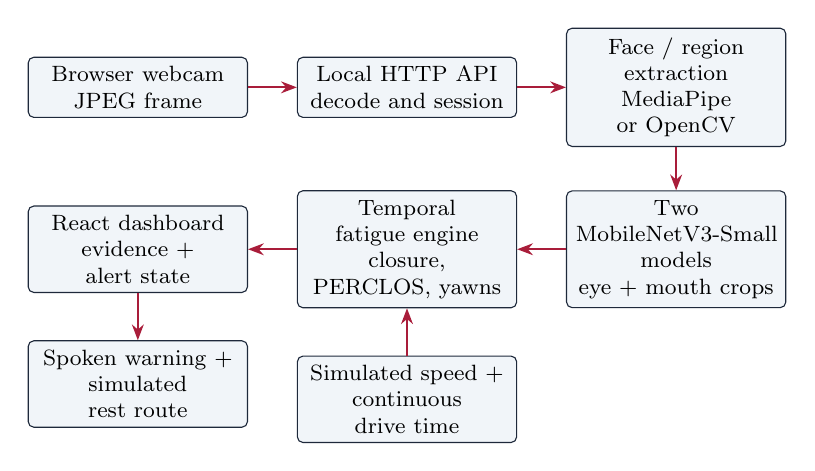
\begin{tikzpicture}[node distance=0.45cm and 0.62cm]
\node[flow] (camera) {Browser webcam\\JPEG frame};
\node[flow,right=of camera] (api) {Local HTTP API\\decode and session};
\node[flow,right=of api] (vision) {Face / region extraction\\MediaPipe or OpenCV};
\node[flow,below=0.55cm of vision] (models) {Two MobileNetV3-Small models\\eye + mouth crops};
\node[flow,left=of models] (engine) {Temporal fatigue engine\\closure, PERCLOS, yawns};
\node[flow,left=of engine] (ui) {React dashboard\\evidence + alert state};
\node[flow,below=0.6cm of engine] (context) {Simulated speed +\\continuous drive time};
\node[flow,below=0.6cm of ui] (alert) {Spoken warning +\\simulated rest route};
\draw[arr] (camera)--(api);\draw[arr] (api)--(vision);\draw[arr] (vision)--(models);
\draw[arr] (models)--(engine);
\draw[arr] (engine)--(ui);\draw[arr] (context)--(engine);\draw[arr] (ui)--(alert);
\end{tikzpicture}}
\par\par\vspace{1pt}
\smallnote{Live inference uses PyTorch CPU checkpoints. ONNX files are exported artifacts.\newline Current browser request interval: 700 ms; timing limitation is discussed later.}
\column{.52\textwidth}
\begin{tabularx}{\linewidth}{L{2.1cm} L{2.1cm} Y}
\toprule\textbf{Module} & \textbf{Input} & \textbf{Processing and output}\\\midrule
Capture & Webcam + telemetry & Encode JPEG; send session request\newline\textbf{Output:} Frame and context\\
Local API & Encoded frame & Decode; orchestrate inference\newline\textbf{Output:} JSON response\\
Face extraction & RGB/BGR image & Locate regions; pad and letterbox\newline\textbf{Output:} Eye/mouth crops\\
Classification & Normalized crops & Two CNN forward passes\newline\textbf{Output:} Class probabilities\\
Temporal policy & Probabilities + time & Track events; scale thresholds\newline\textbf{Output:} Alert and reasons\\
Intervention & Alert response & Display, speak, accept rest route\newline\textbf{Output:} User-facing action\\
\bottomrule\end{tabularx}
\par\vspace{1pt}
\textbf{Separation of responsibilities:} the neural networks classify images; the policy engine maintains history; the interface explains the decision.
\end{columns}

\src{Sources: src/components/DashcamView.jsx; backend/app.py, vision.py, model\_runtime.py and fatigue\_engine.py. Sources: backend/*.py; src/components/*.jsx; src/utils/speech.js.}
\end{frame}

\begin{frame}[t]{Datasets, Preprocessing and Robustness}
\fontsize{10}{11.5}\selectfont
\renewcommand{\arraystretch}{1.06}
\setlength{\tabcolsep}{4pt}
\setlength{\abovedisplayskip}{4pt}
\setlength{\belowdisplayskip}{4pt}
\begin{columns}[T,onlytextwidth]
\column{.49\textwidth}
\textbf{Datasets and attribution}\par\vspace{1pt}
\textbf{UTA Real-Life Drowsiness Dataset}\par\vspace{1pt}
\begin{itemize}\setlength\itemsep{0pt}
\item Official dataset: 60 participants, 180 RGB videos, approximately 30 hours.
\item Original labels: alertness, low vigilance and drowsiness at video level.
\item Project use: eye crops with derived provisional eye-state labels.
\end{itemize}
\href{https://sites.google.com/view/utarldd/home}{Official UTA-RLDD source}\par\vspace{1pt}
\textbf{Yawning Detection Dataset (YawDD)}\par\vspace{1pt}
\begin{itemize}\setlength\itemsep{0pt}
\item Source video tags support normal, talking and yawning scenes in the local pipeline.
\item Project use: eye crops and three-class mouth crops.
\item Dataset DOI: \href{https://doi.org/10.21227/e1qm-hb90}{10.21227/e1qm-hb90}.
\end{itemize}
\href{https://ieee-dataport.org/open-access/yawdd-yawning-detection-dataset}{IEEE DataPort: YawDD dataset}

\par\vspace{1pt}
\smallnote{IEEE DataPort URL: \url{https://ieee-dataport.org/open-access/yawdd-yawning-detection-dataset}}
\column{.49\textwidth}
\textbf{Preprocessing and robustness}\par\vspace{1pt}
\textbf{Training pipeline}\par\vspace{1pt}
\begin{itemize}\setlength\itemsep{0pt}
\item Eye crop: $192\times96$ pixels; mouth: $160\times96$ (width $\times$ height).
\item Horizontal flip with $p=0.5$.
\item Color jitter: brightness/contrast 0.25, saturation 0.10; applied with $p=0.7$.
\item Affine augmentation: $\pm5^\circ$, translation 3\%, scale 0.95--1.05.
\end{itemize}\par\vspace{1pt}
\textbf{Runtime and label preparation}\par\vspace{1pt}
\begin{itemize}\setlength\itemsep{0pt}
\item Preserve crop proportions; fill padding using the crop's median color.
\item Convert BGR to RGB and apply ImageNet normalization.
\item Weak-label preparation uses temporal median EAR/MAR and quality checks.
\item Missing-eye observations have explicit validity and timeout handling.
\end{itemize}\par\vspace{1pt}

\end{columns}

\src{Attribution: Ghoddoosian, Galib and Athitsos, CVPRW 2019; Abtahi et al., YawDD, MMSys 2014, DOI 10.1145/2557642.2563678. See DATASET\_CREDITS.md. Sources: MobileNet notebook training transforms; backend/vision.py; ml/scripts/03\_build\_weak\_labels\_and\_splits\_v2.py. No separate learned denoiser is implemented.}
\end{frame}

\begin{frame}[t]{Dataset Splits, Processing Contribution and Limits}
\fontsize{10}{11.5}\selectfont
\renewcommand{\arraystretch}{1.06}
\setlength{\tabcolsep}{4pt}
\setlength{\abovedisplayskip}{4pt}
\setlength{\belowdisplayskip}{4pt}
\begin{tabularx}{\textwidth}{L{2cm} L{2cm} L{2cm} L{2cm} Y}
\toprule
\textbf{Task} & \textbf{Train crops} & \textbf{Val crops} & \textbf{Test crops} & \textbf{Participants: train / val / test}\\\midrule
Eye & 16,940 & 3,572 & 3,918 & 104 / 23 / 23\\
Mouth & 12,023 & 2,884 & 2,847 & 62 / 14 / 14\\\bottomrule
\end{tabularx}
\par\vspace{1pt}
\begin{itemize}\setlength\itemsep{0pt}
\item Approximately 70/15/15 participant allocation within each dataset; crop ratios vary by participant.
\item \textbf{Verified: zero participant-ID overlap} for train--validation, train--test and validation--test in each task's CSVs.
\item Eye labels use EAR, bilateral agreement and image-quality checks. Mouth labels combine video tags with temporal MAR thresholds.
\item Ambiguous candidates are excluded. Independent ground-truth annotation remains incomplete.
\end{itemize}
\par\medskip
\textbf{Our contribution is the processing workflow, not a newly collected dataset.}
\par\vspace{1pt}
\begin{itemize}\setlength\itemsep{0pt}
\item Generate aspect-preserving eye and mouth crops while retaining participant/video identifiers.
\item Record brightness, blur and landmark geometry for quality-aware weak labelling.
\item Separate original video labels from derived frame-level targets.
\item Provide an annotation queue and local review interface for later human verification.
\item Compare the three architectures on the same task-specific participant splits.
\end{itemize}
\par\vspace{1pt}
\smallnote{This custom hold-out crop-classification protocol differs from UTA-RLDD's recommended five-fold video-level evaluation. Results are therefore not directly comparable to that benchmark.}
\src{Sources: ml/processed\_data\_v2/splits/*.csv and weak\_label\_metadata.json; checked 16 September 2026. Identity checks use (dataset, person\_id), not biometric re-identification. Sources: ml/scripts/01\_extract\_features\_v2.py, 02\_build\_annotation\_queue\_v2.py, 03\_build\_weak\_labels\_and\_splits\_v2.py; \href{https://sites.google.com/view/utarldd/home}{UTA-RLDD evaluation instructions}.}
\end{frame}

\begin{frame}[t]{Deep Learning Architectures: Three Backbones}
\fontsize{10}{11.5}\selectfont
\renewcommand{\arraystretch}{1.06}
\setlength{\tabcolsep}{4pt}
\setlength{\abovedisplayskip}{4pt}
\setlength{\belowdisplayskip}{4pt}
\fontsize{9}{10.5}\selectfont
\begin{columns}[T,onlytextwidth]
\column{.32\textwidth}
\textbf{MobileNetV3-Small}\par\vspace{1pt}
{\centering 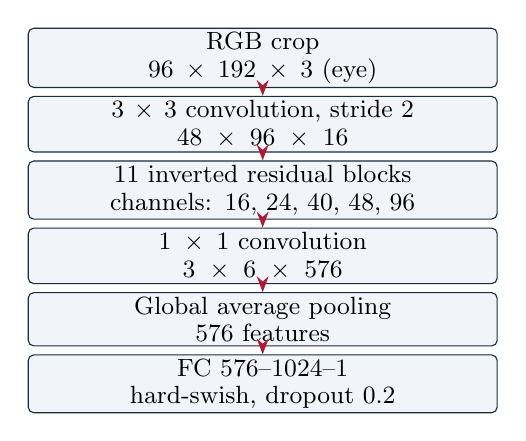
\begin{tikzpicture}[node distance=0.10cm]
\node[flow,text width=5.85cm,font=\fontsize{9}{10}\selectfont,minimum height=.5cm,inner sep=1.5pt] (in) {RGB crop\\$96\times192\times3$ (eye)};
\node[flow,text width=5.85cm,font=\fontsize{9}{10}\selectfont,minimum height=.5cm,inner sep=1.5pt,below=of in] (stem) {$3\times3$ convolution, stride 2\\$48\times96\times16$};
\node[flow,text width=5.85cm,font=\fontsize{9}{10}\selectfont,minimum height=.5cm,inner sep=1.5pt,below=of stem] (bott) {11 inverted residual blocks\\channels: 16, 24, 40, 48, 96};
\node[flow,text width=5.85cm,font=\fontsize{9}{10}\selectfont,minimum height=.5cm,inner sep=1.5pt,below=of bott] (conv) {$1\times1$ convolution\\$3\times6\times576$};
\node[flow,text width=5.85cm,font=\fontsize{9}{10}\selectfont,minimum height=.5cm,inner sep=1.5pt,below=of conv] (pool) {Global average pooling\\576 features};
\node[flow,text width=5.85cm,font=\fontsize{9}{10}\selectfont,minimum height=.5cm,inner sep=1.5pt,below=of pool] (head) {FC 576--1024--1\\hard-swish, dropout 0.2};
\draw[arr](in)--(stem);
\draw[arr](stem)--(bott);
\draw[arr](bott)--(conv);
\draw[arr](conv)--(pool);
\draw[arr](pool)--(head);
\end{tikzpicture}
\par}

\par\vspace{1pt}
\begin{itemize}\setlength\itemsep{0pt}
\item Depthwise convolution reduces spatial-convolution cost; pointwise layers mix channels.
\item Selected blocks use squeeze-and-excitation (SE); residual addition applies when shapes match.
\item Mouth model: separate weights, $96\times160\times3$ input and 3 output logits.
\item Eye head uses sigmoid; mouth head uses softmax. Shapes above are height $\times$ width $\times$ channels.
\end{itemize}
\column{.32\textwidth}
\textbf{EfficientNet-B0}\par\vspace{1pt}
{\centering 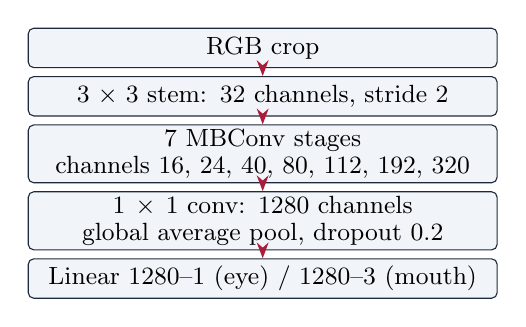
\begin{tikzpicture}[node distance=0.10cm]
\node[flow,text width=5.85cm,font=\fontsize{9}{10}\selectfont,minimum height=.5cm,inner sep=1.5pt] (a) {RGB crop};
\node[flow,text width=5.85cm,font=\fontsize{9}{10}\selectfont,minimum height=.5cm,inner sep=1.5pt,below=of a] (b) {$3\times3$ stem: 32 channels, stride 2};
\node[flow,text width=5.85cm,font=\fontsize{9}{10}\selectfont,minimum height=.5cm,inner sep=1.5pt,below=of b] (c) {7 MBConv stages\\channels 16, 24, 40, 80, 112, 192, 320};
\node[flow,text width=5.85cm,font=\fontsize{9}{10}\selectfont,minimum height=.5cm,inner sep=1.5pt,below=of c] (d) {$1\times1$ conv: 1280 channels\\global average pool, dropout 0.2};
\node[flow,text width=5.85cm,font=\fontsize{9}{10}\selectfont,minimum height=.5cm,inner sep=1.5pt,below=of d] (e) {Linear 1280--1 (eye) / 1280--3 (mouth)};
\draw[arr](a)--(b);
\draw[arr](b)--(c);
\draw[arr](c)--(d);
\draw[arr](d)--(e);
\end{tikzpicture}
\par}

\textbf{MBConv block}\par\vspace{1pt}
Expansion $1\times1$ convolution, depthwise $3\times3$ or $5\times5$, SE channel attention and linear projection. Residual connection where compatible.
\par\vspace{1pt}
\textbf{Stage repeats:} 1, 2, 2, 3, 3, 4, 1.
\par\vspace{1pt}
\par\vspace{1pt}\textbf{Role in this project}\par\vspace{1pt}
An intermediate model-size comparison. We use B0 with the same task crops and training budget; we do not perform a new compound-scaling search.

\column{.32\textwidth}
\textbf{ResNet-18}\par\vspace{1pt}
{\centering 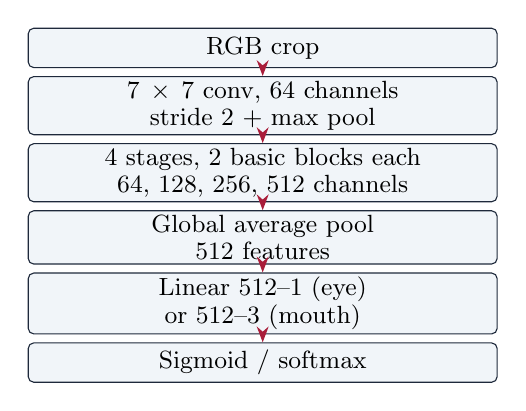
\begin{tikzpicture}[node distance=0.10cm]
\node[flow,text width=5.85cm,font=\fontsize{9}{10}\selectfont,minimum height=.5cm,inner sep=1.5pt] (a) {RGB crop};
\node[flow,text width=5.85cm,font=\fontsize{9}{10}\selectfont,minimum height=.5cm,inner sep=1.5pt,below=of a] (b) {$7\times7$ conv, 64 channels\\stride 2 + max pool};
\node[flow,text width=5.85cm,font=\fontsize{9}{10}\selectfont,minimum height=.5cm,inner sep=1.5pt,below=of b] (c) {4 stages, 2 basic blocks each\\64, 128, 256, 512 channels};
\node[flow,text width=5.85cm,font=\fontsize{9}{10}\selectfont,minimum height=.5cm,inner sep=1.5pt,below=of c] (d) {Global average pool\\512 features};
\node[flow,text width=5.85cm,font=\fontsize{9}{10}\selectfont,minimum height=.5cm,inner sep=1.5pt,below=of d] (e) {Linear 512--1 (eye)\\or 512--3 (mouth)};
\node[flow,text width=5.85cm,font=\fontsize{9}{10}\selectfont,minimum height=.5cm,inner sep=1.5pt,below=of e] (f) {Sigmoid / softmax};
\draw[arr](a)--(b);
\draw[arr](b)--(c);
\draw[arr](c)--(d);
\draw[arr](d)--(e);
\draw[arr](e)--(f);
\end{tikzpicture}
\par}

\par\vspace{1pt}
\textbf{Residual basic block}
\[y=\operatorname{ReLU}\bigl(F(x)+S(x)\bigr)\]
$F$: two $3\times3$ convolutions with batch normalization. $S$: identity or projection for a changed shape.
\par\vspace{1pt}\textbf{Role in this project}\par\vspace{1pt}
A heavier accuracy benchmark. It achieves the highest eye and mouth balanced accuracy among the three tested architectures, with a larger exported model size.

\end{columns}
\src{Architecture: \href{https://arxiv.org/abs/1905.02244}{Howard et al., Searching for MobileNetV3, ICCV 2019}; local torchvision implementation and backend/model\_runtime.py. Architecture: \href{https://arxiv.org/abs/1905.11946}{Tan and Le, EfficientNet, ICML 2019}; local torchvision implementation; efficientnet-b0-comparison.ipynb. Architecture: \href{https://arxiv.org/abs/1512.03385}{He et al., Deep Residual Learning for Image Recognition}; local torchvision implementation; resnet-18-comparison.ipynb.}
\end{frame}

\begin{frame}[t]{Time, Space and Deployment Cost}
\fontsize{10}{11.5}\selectfont
\renewcommand{\arraystretch}{1.06}
\setlength{\tabcolsep}{4pt}
\setlength{\abovedisplayskip}{4pt}
\setlength{\belowdisplayskip}{4pt}
For one convolution: $\mathrm{MACs}=H_oW_oC_o(C_i/g)k^2$, where $g$ is the number of groups. A linear layer uses $C_iC_o$ MACs. Sum over all layers.
\par\vspace{1pt}
\begin{tabularx}{\textwidth}{L{3.1cm} L{2.5cm} L{2cm} L{2cm} Y}
\toprule
\textbf{Architecture} & \textbf{Params, M\newline eye / mouth} & \textbf{Eye\newline M MACs} & \textbf{Mouth\newline M MACs} & \textbf{Both weights\newline FP32 MiB}\\\midrule
MobileNetV3-Small & 1.519 / 1.521 & 21.05 & 17.72 & 11.60 \\
EfficientNet-B0 & 4.009 / 4.011 & 141.66 & 118.15 & 30.59 \\
ResNet-18 & 11.177 / 11.178 & 666.21 & 555.17 & 85.28 \\
\bottomrule
\end{tabularx}
\par\vspace{1pt}

\par\medskip
\begin{columns}[T,onlytextwidth]
\column{.49\textwidth}
\textbf{Complexity interpretation}\par\vspace{1pt}
\begin{itemize}\setlength\itemsep{0pt}
\item Counts use the actual task shapes, batch 1; Conv2d and Linear operations only.
\item Inference compute: $O(\sum_l\mathrm{MACs}_l)$. Inference space: $O(P+A)$ for parameters and live activations.
\item Training also stores gradients/optimizer state; approximately $O(P+BA_{\rm saved})$ space for batch $B$.
\item Temporal PERCLOS computation scans stored intervals: $O(N_w)$ time and $O(N_w+N_y)$ history space.
\end{itemize}
\column{.49\textwidth}
\textbf{Inference cost and deployment}\par\vspace{1pt}
\textbf{Exported eye ONNX size}\par\vspace{1pt}
\begin{tabular}{lr}\toprule
MobileNetV3-Small & 5.80 MiB\\
EfficientNet-B0 & 15.28 MiB\\
ResNet-18 & 42.63 MiB\\\bottomrule
\end{tabular}\par\vspace{1pt}
\par\vspace{1pt}
MobileNet's eye export is approximately $7.35\times$ smaller than ResNet's. Both MobileNet exports total approximately 11.61 MiB.
\par\vspace{1pt}
\smallnote{Exported file size and parameter storage are distinct from total process RAM.}
\par\vspace{1pt}\textbf{Measured local runtime}\par\vspace{1pt}
\begin{tabular}{lr}\toprule
Median & \MedianLatency\ ms\\
95th percentile & \PninetyfiveLatency\ ms\\
Warm-up / timed runs & 20 / 100\\\bottomrule
\end{tabular}\par\vspace{1pt}
\par\vspace{1pt}
Apple M4 CPU, PyTorch 2.13.0, 4 threads, batch 1. Both deployed classifiers plus normalization on synthetic crops.
\par\vspace{1pt}
\smallnote{Excludes face detection, JPEG/API and browser overhead. This is not measured end-to-end camera latency.}

\end{columns}

\src{Reconstructed task architectures, local torchvision, 16 September 2026; presentation\_assets/evidence.json. MACs exclude normalization, activations and pooling. FP32 storage is not peak RAM. Sources: model export records; src/data/modelComparison.js; local benchmark, 16 September 2026, presentation\_assets/evidence.json. Live backend uses PyTorch.}
\end{frame}

\begin{frame}[t]{Algorithms: CNN Forward Pass and Model Training}
\fontsize{10}{11.5}\selectfont
\renewcommand{\arraystretch}{1.06}
\setlength{\tabcolsep}{4pt}
\setlength{\abovedisplayskip}{4pt}
\setlength{\belowdisplayskip}{4pt}
\begin{columns}[T,onlytextwidth]
\column{.49\textwidth}
\textbf{1. CNN forward computation}\par\vspace{1pt}
\begin{enumerate}\setlength\itemsep{0pt}
\item \textbf{Normalize each channel:} $x_c=(I_c/255-\mu_c)/\sigma_c$, with ImageNet $\mu=(.485,.456,.406)$ and $\sigma=(.229,.224,.225)$.
\item \textbf{MobileNet bottleneck:} expand with $1\times1$ convolution (when present), apply channelwise spatial convolution, optional SE, then project:
\[\begin{aligned}
u&=\phi(\mathrm{BN}(W_{\rm exp}*x)),\\
v&=\phi(\mathrm{BN}(W_{\rm dw}*u)),\\
h&=\mathrm{BN}(W_{\rm proj}*\widetilde v).
\end{aligned}\]
\item \textbf{SE, where present:} $z_c=\frac{1}{HW}\sum_{i,j}v_{ijc}$, $a=\operatorname{hard\sigma}(W_2\operatorname{ReLU}(W_1z))$, $\widetilde v_c=a_cv_c$. Otherwise $\widetilde v=v$.
\item \textbf{Residual and pooling:} use $x+h$ when dimensions/stride permit, otherwise $h$; average final spatial features and apply the classifier.
\item \textbf{Output:} eye $p_e=\sigma(z_e)$; mouth $p_k=e^{z_k}/\sum_j e^{z_j}$. Eye closed if $p_e\ge .060$. Yawn if $p_y\ge .355$; otherwise choose the larger non-yawn class probability.
\end{enumerate}
\column{.49\textwidth}
\textbf{2. Training and model selection}\par\vspace{1pt}
\begin{enumerate}\setlength\itemsep{0pt}
\item Split by participant; augment only training images. Initialize ImageNet-pretrained features and replace each output head.
\item Minimize class-weighted binary loss for eyes:
\[\mathcal L_e=-\frac1B\sum_i\left[w_+y_i\log p_i+(1-y_i)\log(1-p_i)\right].\]\[w_+=\sqrt{N_{\rm open}/N_{\rm closed}}.\]
\item For mouths, use weighted cross-entropy with smoothed targets:
\[q_{ik}=.97\,\mathbf1[y_i=k]+.03/3.\]\[\mathcal L_m\propto-\sum_{i,k}w_kq_{ik}\log p_{ik}.\]
\item Backpropagate $g_t=\nabla_\theta\mathcal L$. AdamW updates first/second moments and applies adaptive steps with decoupled weight decay.
\item Save the checkpoint with best validation AP (eye) or macro AP (mouth). Reduce learning rate on a plateau; stop after 4 unimproved epochs.
\item Choose probability thresholds using validation data, lock them, then evaluate the held-out test set once.
\end{enumerate}
\end{columns}

\src{Sources: local torchvision MobileNetV3 implementation; backend/model\_runtime.py. Bias terms omitted in schematic block equations; $\phi$ is the block's ReLU or hard-swish. Sources: all three training notebooks. Mouth weights use normalized square-root inverse frequency; weighted loss reduction follows PyTorch. No test-set threshold tuning is specified.}
\end{frame}

\begin{frame}[t]{Temporal Evidence, Context and Adaptive Alert Rules}
\fontsize{10}{11.5}\selectfont
\renewcommand{\arraystretch}{1.06}
\setlength{\tabcolsep}{4pt}
\setlength{\abovedisplayskip}{4pt}
\setlength{\belowdisplayskip}{4pt}
\begin{columns}[T,onlytextwidth]
\column{.49\textwidth}
\textbf{Accumulate timestamped evidence}
\begin{enumerate}\setlength\itemsep{0pt}
\item Determine whether the face/eye signal is valid and whether $p_e\ge .060$.
\item Track uninterrupted closure; reset when the eye opens, becomes invalid or sample gap exceeds 0.5 s.
\item Compute $P=T_{\rm closed,valid}/T_{\rm valid}$ over up to 60 s. Enable this trigger after 20 s history and $\ge60\%$ valid coverage.
\item Count a yawn after $p_y\ge .355$ persists for 0.75 s; use release hysteresis and a 2 s cooldown.
\end{enumerate}
\textbf{Compute sensitivity}
\[s=s_v s_d,\quad s_v=1+.35\,\operatorname{clip}\!\left(\frac{v-5}{95},0,1\right).\]
\[s_d=\begin{cases}1.00&h<2\\1.10&2\le h<4\\1.25&4\le h<8\\1.40&h\ge8.\end{cases}\]
\smallnote{$v$: simulated km/h; $h$: continuous driving hours. Maximum combined multiplier: $1.35\times1.40=1.89$.}
\par\vspace{1pt}
Keep eye/yawn model thresholds fixed. Change temporal trigger values instead.

\column{.49\textwidth}
\begin{tabularx}{\linewidth}{L{2.2cm} L{3.35cm} Y}
\toprule
\textbf{Signal} & \textbf{Effective threshold} & \textbf{Decision at moving speed}\\\midrule
Sustained closure & Warning $1.5/s$ s; critical $2.5/s$ s & Warning / critical\\
PERCLOS proxy & Warning $\max(.08,.15/s)$; critical $\max(.15,.25/s)$ & Warning / critical after validity gate\\
Yawn events / 5 min & $\max(2,\lceil3/s\rceil)$ events & Advisory\\
No valid eye signal & Longer than 2 s & Sensor unavailable\\
Continuous driving & At least 8 hours & At least advisory\\\bottomrule
\end{tabularx}
\par\vspace{1pt}
\textbf{Example:} at 100 km/h after 4 hours, $s=1.35\times1.25=1.6875$. Closure warning becomes 0.889 s and critical becomes 1.481 s.
\par\vspace{1pt}
\smallnote{The engine selects the highest active severity. Browser controls pause frame requests at 0 km/h. These numerical cutoffs are prototype engineering defaults, not validated physiological limits.}
\end{columns}

\src{Source: backend/fatigue\_engine.py. The current 700 ms browser cadence conflicts with the 500 ms closure continuity limit; see integration limitations. Source: backend/fatigue\_engine.py. At engine speeds below 5 km/h, closure severity is reduced; the UI exposes stopped-vehicle idle behavior.}
\end{frame}

\begin{frame}[t]{Hyperparameters, Input Settings and Justification}
\fontsize{10}{11.5}\selectfont
\renewcommand{\arraystretch}{1.06}
\setlength{\tabcolsep}{4pt}
\setlength{\abovedisplayskip}{4pt}
\setlength{\belowdisplayskip}{4pt}
\begin{columns}[T,onlytextwidth]
\column{.49\textwidth}
\textbf{Training}\par\vspace{1pt}
\renewcommand{\arraystretch}{1.06}
\begin{tabularx}{\linewidth}{L{2.3cm} L{3cm} Y}
\toprule
\textbf{Parameter} & \textbf{Value} & \textbf{Reason for the choice}\\\midrule
Initialization & ImageNet pretrained & Reuse visual features before task adaptation.\\
Optimizer, decay & AdamW / $10^{-4}$ & Adaptive updates with regularization.\\
Learning rates & Backbone $3\times10^{-5}$; head $3\times10^{-4}$ & Adapt the new head faster than pretrained features.\\
Batch size & Train 128; eval 256 & Efficient batches; evaluation avoids backpropagation.\\
Epochs / patience & 15 maximum / 4 & Limit training after validation improvement stalls.\\
LR scheduler & Plateau: factor .5, patience 1 & Reduce steps on stalled AP; LR floor $10^{-6}$.\\
Loss & Weighted BCE / weighted CE & Address class imbalance in eye and mouth tasks.\\
Mouth smoothing & .03 & Soften hard mouth-class targets.\\
Seed & 20260829 & Repeatable experimental setup.\\\bottomrule
\end{tabularx}
\column{.49\textwidth}
\textbf{Input and decision parameters}\par\vspace{1pt}
\begin{tabularx}{\linewidth}{L{2.5cm} L{3cm} Y}
\toprule
\textbf{Setting} & \textbf{Value} & \textbf{Justification / selection basis}\\\midrule
Eye / mouth resolution & $192\times96$ / $160\times96$ & Preserve local facial cues at compact input sizes.\\
Flip / color jitter & $p=.5$ / $p=.7$ & Introduce appearance and orientation variation.\\
Affine transform & $\pm5^\circ$, 3\% shift, 0.95--1.05 scale & Small pose/crop perturbations.\\
Eye probability cutoff & .060 & Validation selection targeting recall $\ge90\%$.\\
Yawn probability cutoff & .355 & Validation selection targeting yawn recall $\ge90\%$.\\
Temporal windows & PERCLOS 60 s; yawns 300 s & Combine short and longer observation histories.\\
Validity gate & 20 s minimum; 60\% valid & Avoid PERCLOS decisions from insufficient evidence.\\
Speed / duration limits & $1.35\times$ / $1.40\times$ & Prototype context-sensitivity design choices.\\\bottomrule
\end{tabularx}
\end{columns}

\src{Sources: training notebooks for all three architectures. Rationales explain design choices; no exhaustive hyperparameter optimization is claimed. Sources: MobileNet notebook; threshold\_metadata.json files; FatigueConfig. Threshold objectives apply to validation, not guaranteed test performance.}
\end{frame}

\begin{frame}[t]{Metrics, Formulas and Literature Benchmark}
\fontsize{10}{11.5}\selectfont
\renewcommand{\arraystretch}{1.06}
\setlength{\tabcolsep}{4pt}
\setlength{\abovedisplayskip}{4pt}
\setlength{\belowdisplayskip}{4pt}
\fontsize{10}{11.5}\selectfont
\renewcommand{\arraystretch}{1.06}
\setlength{\tabcolsep}{3pt}
\setlength{\abovedisplayskip}{3pt}
\setlength{\belowdisplayskip}{3pt}
Positive class = closed eye, or yawn for a one-vs-rest mouth evaluation.
\par\vspace{1pt}
\begin{tabularx}{\textwidth}{L{3.1cm} L{3.4cm} Y}
\toprule
\textbf{Metric / measure} & \textbf{Formula / definition} & \textbf{Purpose and application fit}\\\midrule

Recall & $TP/(TP+FN)$ & Detects positive examples; exposes missed closed eyes/yawns.\\
Precision & $TP/(TP+FP)$ & Positive-prediction reliability; exposes false positives.\\
Specificity & $TN/(TN+FP)$ & Measures rejection of open-eye or non-yawn examples.\\
F1 score & $2TP/(2TP+FP+FN)$ & Balances positive-class precision and recall.\\
Balanced accuracy & $\frac{1}{K}\sum_{k=1}^{K}\mathrm{Recall}_k$ & Gives equal weight to classes despite substantial imbalance.\\
Average precision (AP) & $\sum_n (R_n-R_{n-1})P_n$ & PR-curve summary used for validation checkpoint selection.\\
Macro AP & Mean AP over classes & Gives each mouth class equal importance.\\
PERCLOS proxy & $T_{c,v}/T_v$ & Temporal signal over rolling 60 s; not classifier accuracy.\\
Latency & $t_{\mathrm{end}}-t_{\mathrm{start}}$ & Computation time, distinct from browser sampling rate.\\\bottomrule\end{tabularx}
\par\vspace{1pt}
\smallnote{$TP$: true positive; $FP$: false positive; $TN$: true negative; $FN$: false negative. For binary classification, balanced accuracy = (recall + specificity)/2.}
\par\vspace{1pt}
\textbf{Literature benchmark [1]:} the case study reports MobileNetV3-Small at 94.69\% accuracy, 94.67\% precision and 94.66\% recall on 7,250 Yawn Eye images (four frame classes). These are paper-reported values, not DriveAlert results.
\par\vspace{1pt}
\smallnote{Our three-model comparison uses a shared protocol. The paper's accuracy and our balanced accuracy use different data and protocols; they do not establish a controlled ranking.}

\src{Sources: project evaluation notebooks and saved test\_metrics.json files. Metrics describe provisional labels, not verified fatigue events. Literature values: supplied case study, Section 3.1, paper [1] (Vimala et al., Franklin Open, 2026); standard-paper identity and justification on slide 3.}
\end{frame}

\begin{frame}[t]{Results: Eye States and Mouth Events}
\fontsize{10}{11.5}\selectfont
\renewcommand{\arraystretch}{1.06}
\setlength{\tabcolsep}{4pt}
\setlength{\abovedisplayskip}{4pt}
\setlength{\belowdisplayskip}{4pt}
\fontsize{10}{11.5}\selectfont
\renewcommand{\arraystretch}{1.06}
\setlength{\tabcolsep}{3pt}
\setlength{\abovedisplayskip}{3pt}
\setlength{\belowdisplayskip}{3pt}
\renewcommand{\arraystretch}{1.0}
\textbf{Held-out test: 3,918 crops; 186 closed and 3,732 open.}
\par\vspace{1pt}
\begin{tabularx}{\textwidth}{L{3.2cm} *{5}{>{\centering\arraybackslash}X}}
\toprule
\textbf{Architecture} & \textbf{Balanced acc.} & \textbf{Closed recall} & \textbf{Closed precision} & \textbf{Closed F1} & \textbf{Cutoff}\\\midrule
\rowcolor{HighlightRed}MobileNetV3-Small & 96.93\% & 97.31\% & 58.39\% & 72.98\% & .060\\
EfficientNet-B0 & 96.53\% & 98.39\% & 47.91\% & 64.44\% & .040\\
ResNet-18 & 97.88\% & 98.39\% & 65.12\% & 78.37\% & .025\\\bottomrule
\end{tabularx}
\par\vspace{1pt}

\textbf{Held-out test: 2,847 crops; not-yawn 1,633, talking 935, yawn 279.}
\par\vspace{1pt}
\begin{tabularx}{\textwidth}{L{3.2cm} *{5}{>{\centering\arraybackslash}X}}
\toprule
\textbf{Architecture} & \textbf{3-class balanced acc.} & \textbf{Yawn recall} & \textbf{Yawn precision} & \textbf{Yawn F1} & \textbf{Cutoff}\\\midrule
\rowcolor{HighlightRed}MobileNetV3-Small & 94.41\% & 91.04\% & 96.95\% & 93.90\% & .355\\
EfficientNet-B0 & 94.07\% & 88.89\% & 98.41\% & 93.41\% & .605\\
ResNet-18 & 95.57\% & 93.55\% & 98.86\% & 96.13\% & .650\\\bottomrule
\end{tabularx}
\par\vspace{1pt}
\begin{columns}[T,onlytextwidth]
\column{.49\textwidth}
\begin{itemize}\setlength\itemsep{0pt}
\item ResNet leads balanced accuracy and positive-class F1 among the tested models.
\item MobileNet is 0.95 percentage points below ResNet in balanced accuracy.
\item High recall does not imply high precision: false positive closed-eye frames remain important.
\end{itemize}
\column{.49\textwidth}
\begin{itemize}\setlength\itemsep{0pt}
\item ResNet achieves the best mouth balanced accuracy and yawn recall.
\item EfficientNet's test yawn recall falls below 90\%, despite the validation selection target.
\item MobileNet trades 1.16 percentage points of balanced accuracy for a smaller model.
\end{itemize}
\end{columns}


\src{Sources: eye test\_metrics.json files in ml/models/eye\_v3 and ml/results. Participant-separated evaluation against provisional weak labels. Sources: mouth test\_metrics.json files in ml/models/mouth\_v1 and ml/results. Yawn precision/recall/F1 use yawn-vs-rest; balanced accuracy uses all three classes.}
\end{frame}

\begin{frame}[t]{Confusion Matrices and Error Discussion}
\fontsize{10}{11.5}\selectfont
\renewcommand{\arraystretch}{1.06}
\setlength{\tabcolsep}{4pt}
\setlength{\abovedisplayskip}{4pt}
\setlength{\belowdisplayskip}{4pt}
\setlength{\tabcolsep}{3pt}
\begin{columns}[T,onlytextwidth]
\column{.45\textwidth}
\textbf{MobileNet eye}\par\vspace{1pt}
\begin{tabular}{lrr}
\toprule
True $\backslash$ predicted & Open & Closed\\\midrule
Open & \cellcolor{CardBg}3603 & 129\\
Closed & 5 & \cellcolor{CardBg}181\\\bottomrule
\end{tabular}
\par\vspace{1pt}
\begin{itemize}\setlength\itemsep{2mm}
\item 5 of 186 closed examples missed.
\item 129 of 310 closed predictions are false positives against weak labels.
\item Temporal filtering needs separate event-level evaluation.
\end{itemize}
\column{.52\textwidth}
\textbf{MobileNet mouth}\par\vspace{1pt}
\begin{tabular}{lrrr}
\toprule
True $\backslash$ predicted & Not-yawn & Talking & Yawn\\\midrule
Not-yawn & \cellcolor{CardBg}1586 & 47 & 0\\
Talking & 38 & \cellcolor{CardBg}889 & 8\\
Yawn & 0 & 25 & \cellcolor{CardBg}254\\\bottomrule
\end{tabular}
\par\vspace{1pt}
\begin{itemize}\setlength\itemsep{2mm}
\item 25 yawn examples classified as talking.
\item 8 talking examples classified as yawn.
\item Classification scores do not measure fatigue-event sensitivity or warning delay.
\end{itemize}
\end{columns}
\src{Sources: drivealert\_eye\_v3\_test\_metrics.json and drivealert\_mouth\_v1\_test\_metrics.json. Rows are ground labels in the saved provisional evaluation.}
\end{frame}

\begin{frame}[t]{Training Curves: Validation AP and MobileNet Loss}
\fontsize{10}{11.5}\selectfont
\renewcommand{\arraystretch}{1.06}
\setlength{\tabcolsep}{4pt}
\setlength{\abovedisplayskip}{4pt}
\setlength{\belowdisplayskip}{4pt}
\fontsize{10}{11.5}\selectfont
\renewcommand{\arraystretch}{1.06}
\setlength{\tabcolsep}{3pt}
\setlength{\abovedisplayskip}{3pt}
\setlength{\belowdisplayskip}{3pt}
\begin{columns}[T,onlytextwidth]
\column{.49\textwidth}\centering\textbf{Eye: positive-class AP}
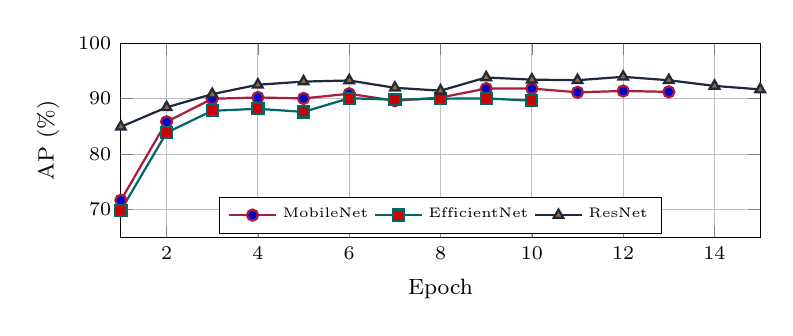
\begin{tikzpicture}
\begin{axis}[width=9.7cm,height=4.05cm,xlabel=Epoch,ylabel={AP (\%)},xmin=1,xmax=15,ymin=65,ymax=100,grid=major,tick label style={font=\scriptsize},label style={font=\footnotesize},legend columns=3,legend style={font=\tiny,at={(.5,.02)},anchor=south},legend cell align=left]
\addplot+[color=AmritaRed,mark=*,thick] coordinates {(1,71.7082) (2,85.8380) (3,89.9802) (4,90.2142) (5,90.0469) (6,90.8847) (7,89.6239) (8,90.2010) (9,91.8239) (10,91.8208) (11,91.1488) (12,91.3843) (13,91.2295)};\addlegendentry{MobileNet}
\addplot+[color=teal!80!black,mark=square*,thick] coordinates {(1,69.9045) (2,83.8732) (3,87.8233) (4,88.1748) (5,87.6143) (6,90.0768) (7,89.8192) (8,89.9943) (9,90.0549) (10,89.6252)};\addlegendentry{EfficientNet}
\addplot+[color=DarkSlate,mark=triangle*,thick] coordinates {(1,84.9289) (2,88.4397) (3,90.8148) (4,92.5096) (5,93.0760) (6,93.2747) (7,91.9555) (8,91.4402) (9,93.8164) (10,93.4244) (11,93.3271) (12,93.9350) (13,93.3136) (14,92.3011) (15,91.6667)};\addlegendentry{ResNet}

\end{axis}\end{tikzpicture}
\column{.49\textwidth}\centering\textbf{Mouth: macro AP}
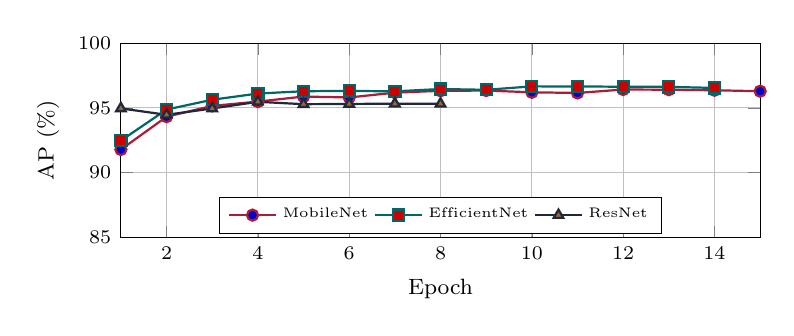
\begin{tikzpicture}
\begin{axis}[width=9.7cm,height=4.05cm,xlabel=Epoch,ylabel={AP (\%)},xmin=1,xmax=15,ymin=85,ymax=100,grid=major,tick label style={font=\scriptsize},label style={font=\footnotesize},legend columns=3,legend style={font=\tiny,at={(.5,.02)},anchor=south},legend cell align=left]
\addplot+[color=AmritaRed,mark=*,thick] coordinates {(1,91.7901) (2,94.3229) (3,95.1572) (4,95.4878) (5,95.8782) (6,95.8083) (7,96.1788) (8,96.3196) (9,96.3410) (10,96.2056) (11,96.1551) (12,96.4205) (13,96.4054) (14,96.3629) (15,96.2897)};\addlegendentry{MobileNet}
\addplot+[color=teal!80!black,mark=square*,thick] coordinates {(1,92.4784) (2,94.8747) (3,95.6325) (4,96.1092) (5,96.2890) (6,96.3138) (7,96.2795) (8,96.4597) (9,96.3990) (10,96.6628) (11,96.6587) (12,96.6345) (13,96.6257) (14,96.5438)};\addlegendentry{EfficientNet}
\addplot+[color=DarkSlate,mark=triangle*,thick] coordinates {(1,94.9631) (2,94.4699) (3,94.9565) (4,95.4727) (5,95.2886) (6,95.3077) (7,95.3269) (8,95.3214)};\addlegendentry{ResNet}

\end{axis}\end{tikzpicture}
\end{columns}
\begin{columns}[T,onlytextwidth]
\column{.49\textwidth}\centering\textbf{Eye: weighted binary loss}
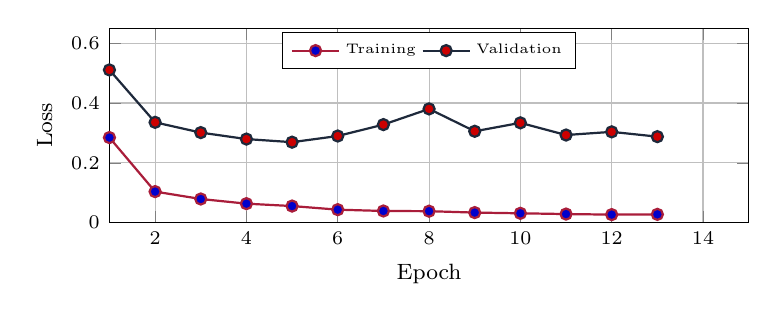
\begin{tikzpicture}
\begin{axis}[width=9.7cm,height=4.05cm,xlabel=Epoch,ylabel=Loss,xmin=1,xmax=15,ymin=0,ymax=.65,grid=major,tick label style={font=\scriptsize},label style={font=\footnotesize},legend columns=2,legend style={font=\tiny,at={(.5,.98)},anchor=north}]
\addplot+[color=AmritaRed,mark=*,thick] coordinates {(1,0.28430) (2,0.10360) (3,0.07891) (4,0.06327) (5,0.05527) (6,0.04322) (7,0.03878) (8,0.03813) (9,0.03344) (10,0.03104) (11,0.02852) (12,0.02664) (13,0.02750)};\addlegendentry{Training}
\addplot+[color=DarkSlate,mark=*,thick] coordinates {(1,0.51053) (2,0.33526) (3,0.30094) (4,0.27929) (5,0.26892) (6,0.28951) (7,0.32767) (8,0.38017) (9,0.30536) (10,0.33356) (11,0.29285) (12,0.30345) (13,0.28734)};\addlegendentry{Validation}

\end{axis}\end{tikzpicture}
\column{.49\textwidth}\centering\textbf{Mouth: weighted multiclass loss}
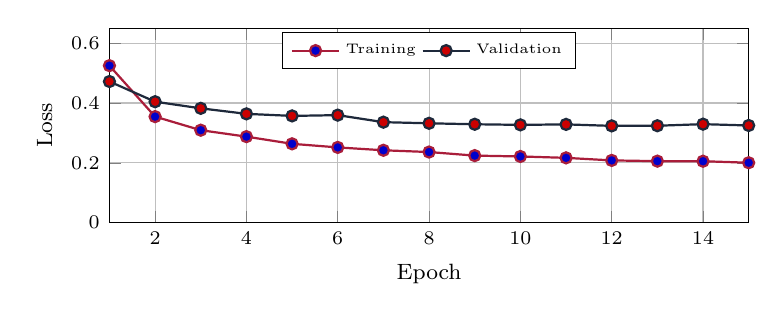
\begin{tikzpicture}
\begin{axis}[width=9.7cm,height=4.05cm,xlabel=Epoch,ylabel=Loss,xmin=1,xmax=15,ymin=0,ymax=.65,grid=major,tick label style={font=\scriptsize},label style={font=\footnotesize},legend columns=2,legend style={font=\tiny,at={(.5,.98)},anchor=north}]
\addplot+[color=AmritaRed,mark=*,thick] coordinates {(1,0.52480) (2,0.35436) (3,0.30899) (4,0.28741) (5,0.26341) (6,0.25143) (7,0.24181) (8,0.23592) (9,0.22398) (10,0.22112) (11,0.21647) (12,0.20792) (13,0.20548) (14,0.20523) (15,0.20014)};\addlegendentry{Training}
\addplot+[color=DarkSlate,mark=*,thick] coordinates {(1,0.47183) (2,0.40423) (3,0.38207) (4,0.36363) (5,0.35679) (6,0.35934) (7,0.33584) (8,0.33204) (9,0.32883) (10,0.32679) (11,0.32840) (12,0.32342) (13,0.32388) (14,0.32918) (15,0.32476)};\addlegendentry{Validation}

\end{axis}\end{tikzpicture}
\end{columns}

\smallnote{Curves stop at each recorded run's final epoch. Checkpoints are selected by validation AP, not by the test scores.}
\smallnote{Training loss falls below validation loss. This motivates checkpoint selection and early stopping; low training loss alone does not establish generalization.}

\src{Sources: six saved history.csv files. Native editable plot coordinates are stored in presentation\_assets/*\_ap\_plot.tex. Sources: MobileNet eye and mouth history.csv files. Different tasks/loss functions should not be compared by absolute loss magnitude.}
\end{frame}

\begin{frame}[t]{UI: Application Entry and Model Comparison}
\fontsize{10}{11.5}\selectfont
\renewcommand{\arraystretch}{1.06}
\setlength{\tabcolsep}{4pt}
\setlength{\abovedisplayskip}{4pt}
\setlength{\belowdisplayskip}{4pt}
\fontsize{10}{11.5}\selectfont
\renewcommand{\arraystretch}{1.06}
\setlength{\tabcolsep}{3pt}
\setlength{\abovedisplayskip}{3pt}
\setlength{\belowdisplayskip}{3pt}
\begin{columns}[T,onlytextwidth]
\column{.49\textwidth}
\textbf{Application Entry}\par\vspace{1pt}
\centering
\includegraphics[width=\linewidth,height=7cm,keepaspectratio,trim=0 347bp 0 0,clip]{ui_landing.jpg}
\par\vspace{1pt}
\begin{itemize}\setlength\itemsep{0pt}
\item Launch the simulator for monitoring and examiner controls.
\item Open model comparison to inspect architecture tradeoffs and held-out metrics.
\end{itemize}
\column{.49\textwidth}
\textbf{Model Comparison}\par\vspace{1pt}
\centering
\includegraphics[width=\linewidth,height=7cm,keepaspectratio]{ui_comparison.jpg}
\end{columns}


\src{Actual browser capture of src/components/LandingPage.jsx, 16 September 2026. Captured entry controls; no live detection is shown. Actual model-comparison interface. The screen compares eye metrics and exposes the weak-label evaluation note. Sources: ModelComparison.jsx and src/data/modelComparison.js.}
\end{frame}

\begin{frame}[t]{UI Screen: Monitoring Dashboard}
\fontsize{10}{11.5}\selectfont
\renewcommand{\arraystretch}{1.06}
\setlength{\tabcolsep}{4pt}
\setlength{\abovedisplayskip}{4pt}
\setlength{\belowdisplayskip}{4pt}
\centering
\includegraphics[width=.96\textwidth,height=9.5cm,keepaspectratio]{ui_dashboard.jpg}
\src{Actual browser capture: stopped-vehicle idle state; camera permission unavailable in this capture. Probability and temporal evidence panels are visible; this is not a camera-detection result.}
\end{frame}

\begin{frame}[t]{UI: Spoken Intervention and Simulated Rest Route}
\fontsize{10}{11.5}\selectfont
\renewcommand{\arraystretch}{1.06}
\setlength{\tabcolsep}{4pt}
\setlength{\abovedisplayskip}{4pt}
\setlength{\belowdisplayskip}{4pt}
\fontsize{10}{11.5}\selectfont
\renewcommand{\arraystretch}{1.06}
\setlength{\tabcolsep}{3pt}
\setlength{\abovedisplayskip}{3pt}
\setlength{\belowdisplayskip}{3pt}
\begin{columns}[T,onlytextwidth]
\column{.49\textwidth}
\textbf{Spoken Intervention and Rest Offer}\par\vspace{1pt}
\centering
\includegraphics[width=\linewidth,height=7cm,keepaspectratio]{ui_intervention.jpg}
\column{.49\textwidth}
\textbf{Simulated Route and Examiner Controls}\par\vspace{1pt}
\centering
\includegraphics[width=\linewidth,height=7cm,keepaspectratio]{ui_reroute.jpg}
\end{columns}


\src{Actual examiner-triggered microsleep scenario. Buttons support voice-warning playback, accepting a simulated rest route or continuing monitoring. This screen is not evidence of a detected fatigue event. Actual browser capture after accepting the examiner scenario. Route/distance are hardcoded demonstration values. Speed/duration sliders and scenario controls supply simulated context.}
\end{frame}

\begin{frame}[t]{Validation, Project Outcomes and Next Steps}
\fontsize{10}{11.5}\selectfont
\renewcommand{\arraystretch}{1.06}
\setlength{\tabcolsep}{4pt}
\setlength{\abovedisplayskip}{4pt}
\setlength{\belowdisplayskip}{4pt}
\fontsize{10}{11.5}\selectfont
\renewcommand{\arraystretch}{1.06}
\setlength{\tabcolsep}{3pt}
\setlength{\abovedisplayskip}{3pt}
\setlength{\belowdisplayskip}{3pt}
\begin{columns}[T,onlytextwidth]
\column{.49\textwidth}
\textbf{Validation evidence and observed status}\par\vspace{1pt}
\textbf{Saved model evaluation:} Eye/mouth metrics, predictions, threshold reports and learning curves available.\par\vspace{2pt}
\textbf{Backend test suite:} 10 tests passed locally on 16 September 2026.\par\vspace{2pt}
\textbf{Participant separation:} No shared recorded participant IDs across the task split pairs.\par\vspace{2pt}
\textbf{Closure integration:} Browser interval 700 ms exceeds engine's 500 ms continuity limit. Synthetic 700 ms closed-eye samples repeatedly reset closure duration.\par\vspace{2pt}
\textbf{Real-world validation:} No independently labelled live-driving event benchmark or false-alert/hour result.\par\vspace{2pt}
\par\vspace{1pt}
\textbf{Required before the camera demonstration:} reconcile frame timing and the continuity policy, then test sustained closure and dropped-frame behavior end to end.
\par\vspace{1pt}
\smallnote{Unit tests cover isolated behavior; they do not resolve the browser/engine cadence mismatch. Manual scenario buttons demonstrate the interface only.}
\column{.49\textwidth}
\textbf{Completed project components}\par\vspace{1pt}
\begin{itemize}\setlength\itemsep{0pt}
\item Three architecture experiments, two classification tasks and saved evaluation artifacts.
\item Local inference API, face-region extraction and temporal decision engine.
\item React dashboard, voice-warning controls and simulated routing workflow.
\end{itemize}
\textbf{Remaining validation and review work}\par\vspace{1pt}
\begin{itemize}\setlength\itemsep{0pt}
\item Retain the full case study for paper details and journal-listing evidence.
\item Fix and verify the closure timing integration.
\item Independently annotate events and test false alerts, delays, lighting and occlusion.
\item Compare fixed, confidence-adaptive and context-adaptive policies before claiming improved outcomes.
\end{itemize}

\end{columns}


\src{Sources: backend/tests; DashcamView.jsx:134; fatigue\_engine.py:43 and closure logic. Application behavior was not changed for this presentation update. Prototype conclusion: competitive crop-classification results and an implemented application workflow; production driving effectiveness remains unverified.}
\end{frame}

\begin{frame}[t]{References and Reproducibility}
\fontsize{10}{11.5}\selectfont
\renewcommand{\arraystretch}{1.06}
\setlength{\tabcolsep}{4pt}
\setlength{\abovedisplayskip}{4pt}
\setlength{\belowdisplayskip}{4pt}
\footnotesize
\begin{enumerate}\setlength\itemsep{2mm}
\item Howard et al. \textit{Searching for MobileNetV3}. ICCV, 2019. \href{https://arxiv.org/abs/1905.02244}{arXiv:1905.02244}.
\item Tan and Le. \textit{EfficientNet: Rethinking Model Scaling for Convolutional Neural Networks}. ICML, 2019. \href{https://arxiv.org/abs/1905.11946}{arXiv:1905.11946}.
\item He et al. \textit{Deep Residual Learning for Image Recognition}. \href{https://arxiv.org/abs/1512.03385}{arXiv:1512.03385}.
\item Ghoddoosian, Galib and Athitsos. \textit{A Realistic Dataset and Baseline Temporal Model for Early Drowsiness Detection}. CVPRW, 2019. \href{https://arxiv.org/abs/1904.07312}{arXiv:1904.07312}.
\item Abtahi et al. \textit{YawDD: A Yawning Detection Dataset}. MMSys, 2014. \href{https://doi.org/10.1145/2557642.2563678}{doi:10.1145/2557642.2563678}.
\end{enumerate}
\par\vspace{1pt}
\textbf{Project evidence:} \texttt{ml/notebooks/}, \texttt{ml/models/}, \texttt{ml/results/}, \texttt{ml/processed\_data\_v2/splits/}, \texttt{backend/} and \texttt{src/}.
\par\vspace{1pt}
\textbf{Presentation evidence:} plots, real UI captures and local measurements in \texttt{presentation\_assets/}. The accompanying \textit{DriveAlert Case Study Review 2: 15 Papers} contains the full journal bibliography; its reference numbers apply to slides 3 and 12.
\src{Repository: \href{https://github.com/krishnans4132/DriveAI}{github.com/krishnans4132/DriveAI}. Literature benchmarks are attributed separately from locally measured project results.}
\end{frame}

\end{document}
